\subsection{Electromagnetic Calorimeter} 
\label{sec:ecal}

The Ecal, depicted in Fig. \ref{fig:ecal}, consists of $442$ lead-tungstate PbWO$_4$ crystals with avalanche photodiode (APD) readout and amplifiers, Figure \ref{fig:module}. Those have all similarly short pulse widths, so that they can run at very high rates. Indeed, the expected high radiation and high rate environment, together with a high magnetic field in close proximity, essentially imposed lead-tungstate (PbWO$_4$) crystals with APD readout. The lead tungsten (PbWO$_4$) crystals are taken from the Inner Calorimeter (IC) of the JLab CLAS detector, which was originally build in IPN Orsay (France) and run for 10 years with success. Crystals in the ECal are arranged in two modules, see Fig. \ref{fig:ecal}. There are 5 layers in each module; four layers have $46$ crystals and one has $37$. The ECal is mounted downstream of the analyzing dipole magnet at the distance of about $137$ cm from the upstream edge of the magnet. The two ECal modules are positioned just above and below the ECal vacuum chamber, through which the beam and the wall of flame passes in vacuum. At its closest point, the edge of the crystal is at $3.7$ cm from the beam. In order to maintain stable performance of the PbWO$_4$ calorimeter, the crystals and APDs are enclosed within a temperature stabilized environment, held constant at the level of 1\!\char23F. The expected energy resolution of the system from operational experience with the IC is $\sigma_E/E \sim 4.5\%/\sqrt{E}$ (GeV). As in the IC, PbWO$_4$ modules are connected to a motherboard that provides power and transmits signals from individual APDs and pre-amplifier boards. The ECal data is digitized using the JLAB FADC250, a 250 MHz flash ADC developed for the 12 GeV Upgrade. The full analogue information from the FADCs coupled with the spatial and time information of each module are available to the trigger system, which uses energy deposition, position, timing, and energy-position correlation to reduce the trigger rate to a manageable $\sim 30$ kHz (see Section \ref{sec:triggerdaq} for details).

\begin{figure*}[t]
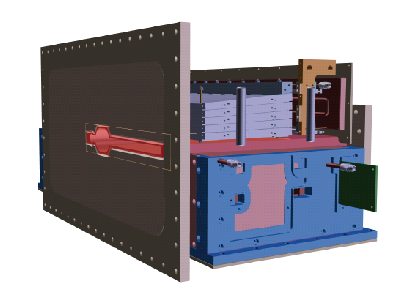
\includegraphics[width=\textwidth]{ecal/ECal.png}
\caption{\small{Arrangement of Ecal crystals. Two modules are positioned above and below the beam plane. Each module has 5 layers. There are 46 crystals in each layer, with exception of layers closest to the beam plane where 9 crystals are missing to allow larger opening for outgoing electron and photon beams.}}\label{fig:ecal}
\end{figure*}

\begin{figure*}[t]
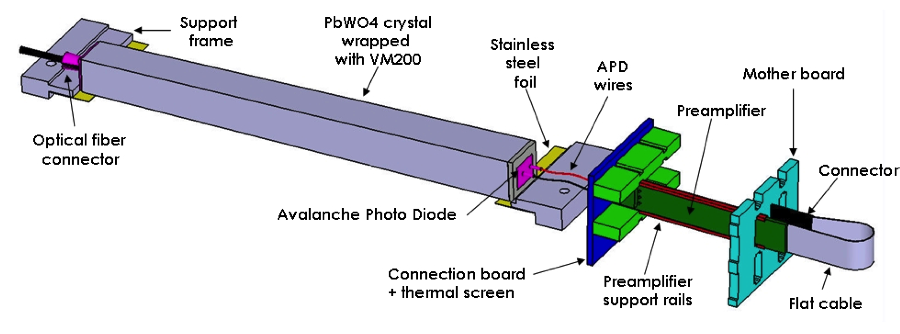
\includegraphics[width=\textwidth]{ecal/ecal_module.png}
\caption{\small{ECal module composed of 16 cm long lead-ungstate crystal, Avalanche Photo Diode, and a peramplifier board.}}\label{fig:module}
\end{figure*}

Calorimeter described above was built and used during the HPS test run in April-May of 2012. For the first time, for the readout and the trigger system for a calorimeter in real experiment JLAB FADC250s were used. The trigger algorithm was designed to satisfy HPS event selection criteria and was based on a newly developed FPGA based trigger processors. With photon beams, only limited aspects of the whole system were tested. Critical parts of the ECal performed well during the test ran and the min goals of the run were achieved (see Section \ref{sec:testrun2012} for details). While ECal performance during the test run was satisfactory, several areas are in need for improvements. In the following subsections planned improvements to the existing ECal are described.   

\subsubsection{Improvements to the existing calorimeter}

There are no plans for major mechanical changes. The crystals, support frames, and thermal enclouser will stay unchanged. The most of changes are related to the signal readout chain and they are based on the operational experience with ECal and FADC250. Below details of modifications/improvements are given: 

\begin{enumerate}
\item {\bf Replacing the ECal mounting system} - 
During the test run ECal was mounted on the Hall-B pair spectrometer mount rails together with the pair spectrometer hodoscopes. The ECal vacuum chamber was not install and the fine alignment of ECal was not necessary. Due to limited space on the mounting rails and the no need for a mounting system with fine adjustments, ECal was hang from the mount rails using simply long threaded roads. This system must be replaced with a more sturdy and better adjustable (horizontally and vertically) system in order to properly align ECal in close contact with the ECal vacuum chamber

\item {\bf Modifications to the side brackets to accommodate fiber bundles for light monitoring system} -
The light monitoring system was not used during the test run. While design of the ECal enclosure is done in a way that it will will accommodated optical fibers connected in front face of crystals, side plates that hold crystal frames does not have inlets for light monitoring fiber bundle. Space is available on the side plates. Modification will require making holes and placing transition connectors  
    
\item {\bf Modification of motherboards} - One of issues we faced during the test run was the noise on motherboards. Missing channels seen on the performance figures in Section \ref{sec:performace} are largely due to switching off noisy channels since there was not time for debugging them. The new motherboards will be designed and build to resolve issues encountered during the test run. One of options in discussion is to replace long motherboards with shorter ones with power and signal connectors located on the top (for top module) and bottom (for bottom module) of the thermal enclosure

\item {\bf Get read of signal splitting} - From experience gained with JLAB FADC250 by HPS group as well as other groups at JLAB working on detector developments in different group, it is evident that with right firmware they can be used for time measurements as well as can work as scalers. Present ECal readout configuration uses signal splitters to split APD signal after preamplifier in 2:1 ratio then sends $2/3$ of the signal to a discriminator that has built-in scalers and feeds the TDC channel. The 1/3 of the signal goes to FADC for energy measurements. Removing the split will increase signal on FADC input by $\time 2$. This will allow to lower gain of amplifiers Using the FADC250 for time measurements and as a scaler is planned for other detectors at JLAB 
 
\item {\bf New preamplifiers} - with increased signal strength at the input of FADC by $\time 2$ after eliminating the signal splitter, preamplifier gains can be lowered the same amount without loosing in resolution. Lowering the preamplifier gains will reduce the noise and will allow to bring down thresholds on individual channels. The impact of lower noise/threshold system is twofold - first it will improve resolution, the second it will allow to setup MIP calibration system for ECal modules while they are installed. As shown in studies performed by HPS collaborators from INFN Genova, with low noise, low threshold system MIP energy deposition can be seen in the module for transverse cosmic muons, see Figure \ref{fig:mip10x10} and explanations below

\item {\bf Light monitoring system}

For an experiment like HPS, where backgrounds must be well understood and need to be strongly suppressed, the trigger bias can be an important issue. In particular, having a stable and known thresholds at the trigger readout are necessary in order to avoid the bias in the event selection. The uniformity of the trigger response and the stability can be achieved with the installation of an online gain monitoring system. This system will introduce short light pulses in the front of the crystals. Crystals have fiber holder glued on front face and implementation of the system will not require modification of crystals and wrapping. 

Optical fibers will be used to transmit light from the source to the crystals to test response of APDs. The response of the system will therefore be sensitive to both transparency losses of crystals due to a possible radiation damage and gain variations of APDs. Such a system has been developed for several experiments (CMS at CERN for instance) with various light sources. The system for ECal will be developed in IPN Orsay during 2013 and in the first half of 2014, to be ready for installation at JLAB for the commissioning run at the end of 2014. We choose, for their low cost, to use two different mono-color LEDs as light sources to monitor responses of each module. A blue light, which corresponds to the domain of the crystal emission, and is very sensitive to the presence of color centers, produced by radiation damage. This light source is very useful to test variations of the response in the main domain of the emission. Impurities can anneal at room temperature and such monitoring can be sensitive to increasing of output as well, when the radiation exposure is reduced for a long period of time. A red colored light, less sensitive to the color centers, permits monitoring the APD gains more directly and thereby separates effects of APD and electronics from the crystal transparency, and provide clear information on the state of the electronics. The main challenge for the system is to guarantee stability at a level better than a couple percent to be able to identify and to adapt to the transparency variations. The test of the system will be carried-on at IPN Orsay, in order to guarantee its efficiency and also to test radiation resistance of the various materials

\item {\bf New low-voltage power supply} - the existing low voltage power supply is a manually controlled, single output power supply that feeds four motherboards through custom-made patch panel. Inability of controlling voltage supply to preamplifiers at different parts of the ECal and remotely controlling/resetting them is a big disadvantage, requires frequent access to the Hall, especially in the commissioning phase. Available new low voltage power supplies are much more flexible, the one that is the most suitable for ECal APD preamplifiers is WEINER MPV 8008LD. This power supply will be used at JLAB and the control software exists.     

\end{enumerate}
  

\subsubsection{Possibilities with new APDs} 

The second major improvement to be done for the calorimeter consists in the implementation of new APDs, by replacing old $5\times 5$ mm$^2$ APDs with $10\times 10$ mm$^2$, Hamamatsu S8664-1010. The renewal of the APDs will resolve two issues with present modules of HPS calorimeter. First, new APDs from Hamamatsu have much better performance than the ones which are now installed on lead-tungstate crystals. Data from Hamamatsu shows that APDs made from the same wafer have excellent uniformity. With $\pm 10\%$ known uniformity at the gain of $100$, variations in bias voltage are $\sim 4.5$ V. Moreover, data provided for samples of 1300 the bias voltage difference is ~50 V, when for APDs now we have ($442$ pieces) the voltage difference is more than $100$ V. The bias voltage to APDs is not supplied individually, a group of APDs are supplied the same bias voltage and but they supplied to a group and therefore with new APDs that have much smaller voltage-gain variations much better uniformity in the response of the calorimeter modules in the trigger can be achieved. 

Second, a $4$ times larger readout area will ensure $4$ times more light collection and therefore $4$ time larger signal from APDs. This will allow the use of different amplifier modules with lower gain that in turn will decrease electronic noise. Tests performed for another calorimeter, now in production at INFN Genova for JLAB Hall-B, showed that the same type of amplifier boards with factor 2 lower gains have noise level on the order of $<5$ MeV. Minimum ionizing energy deposition in PbWO$_4$ crystals of HPS calorimeter from cosmic muons passing through perpendicular to the crystal axis is of $\sim 15$ MeV. If energy thresholds can be moved close to $5$ MeV, then MIP peak will be seen and calorimeter can be calibrated and monitored with cosmic muons. The HPS collaborators from INFN group made the first tests with HPS crystals using Hamamtsu $10\times 10$ mm$^2$ APDs and a new amplifier board. In Figure \ref{fig:mip10x10} charge distribution of the single crystal system is shown for $5\times 5$ mm$^2$ (left) and $10\times 10$ mm$^2$ (right) APDs. The red line histogram is for all events triggered by scintillation telescope placed above and below the crystal. The black line histogram corresponds to charge distribution within $100$ ns of coincidence time. The MIP peak is clearly visible and well isolated from the pedestal (noise) for S8664-1010 APD readout. For  S8664-55 APD MIP signal is also seen, but the MIP charge distribution is under the noise peak and does not have well defined peak position. Possibility of detecting MIP particles traversing the system in perpendicular direction will allow to calibrate the modules with cosmic muons while they are installed in the HPS system. This is a great advantage and together with light monitoring system will ensure stable and reliable performance of the ECal and the trigger system. In addition to the possibility of calibrating the modules with cosmic muons (MIP calibration), the lower noise will allow to lower the acquisition thresholds and improve the energy resolution. The new amplifier boards have to be designed to work with new APDs. 

\begin{figure*}[t]
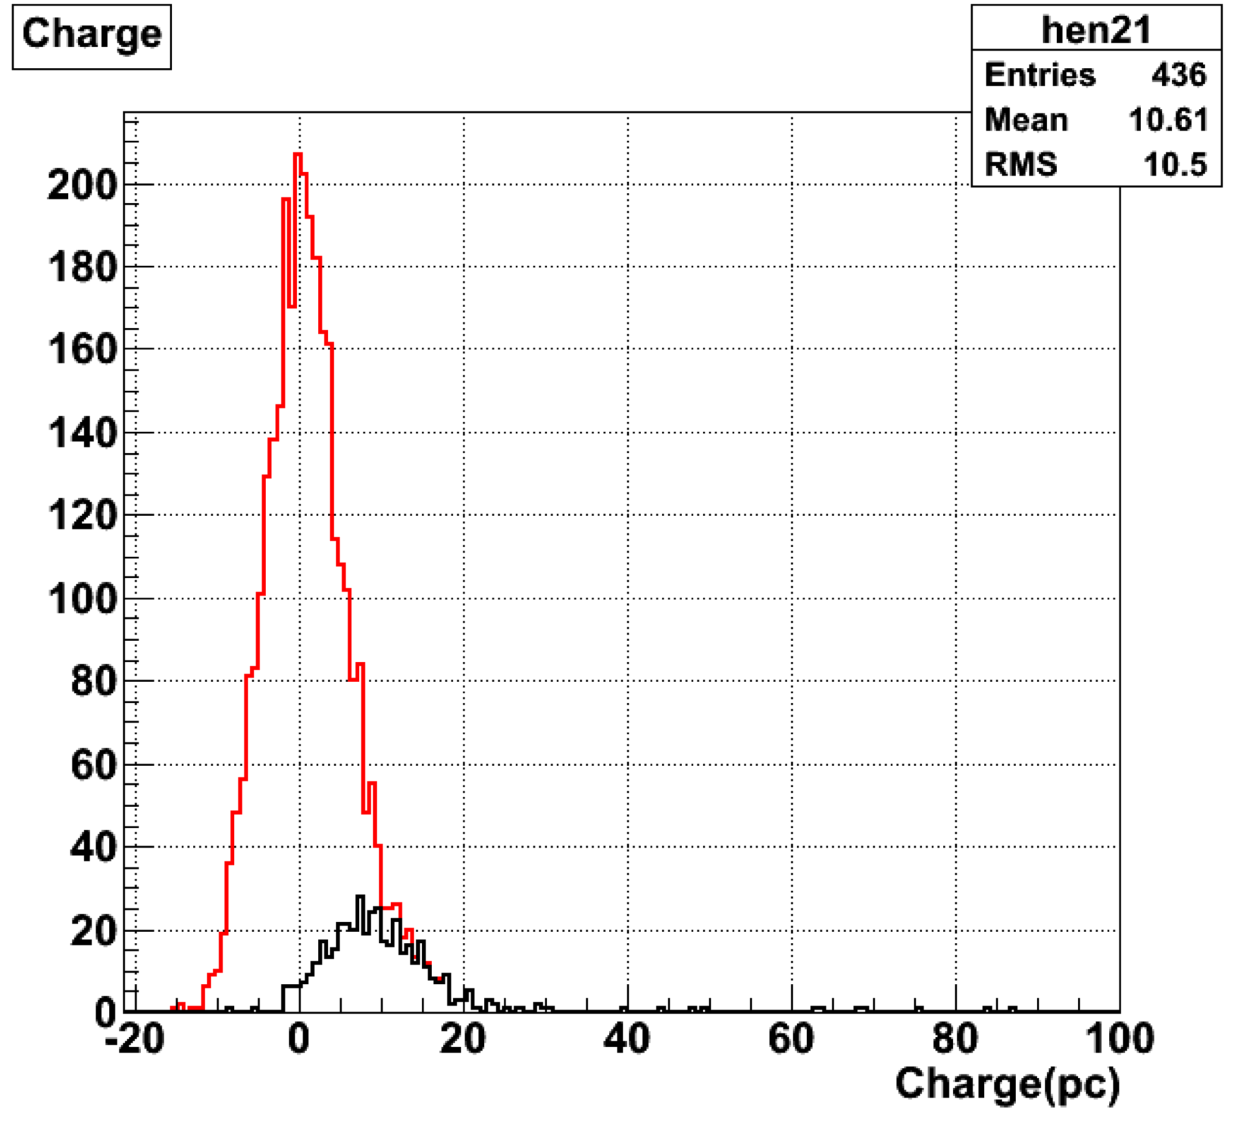
\includegraphics[scale=0.37]{ecal/MIP_5x5_APD.png}
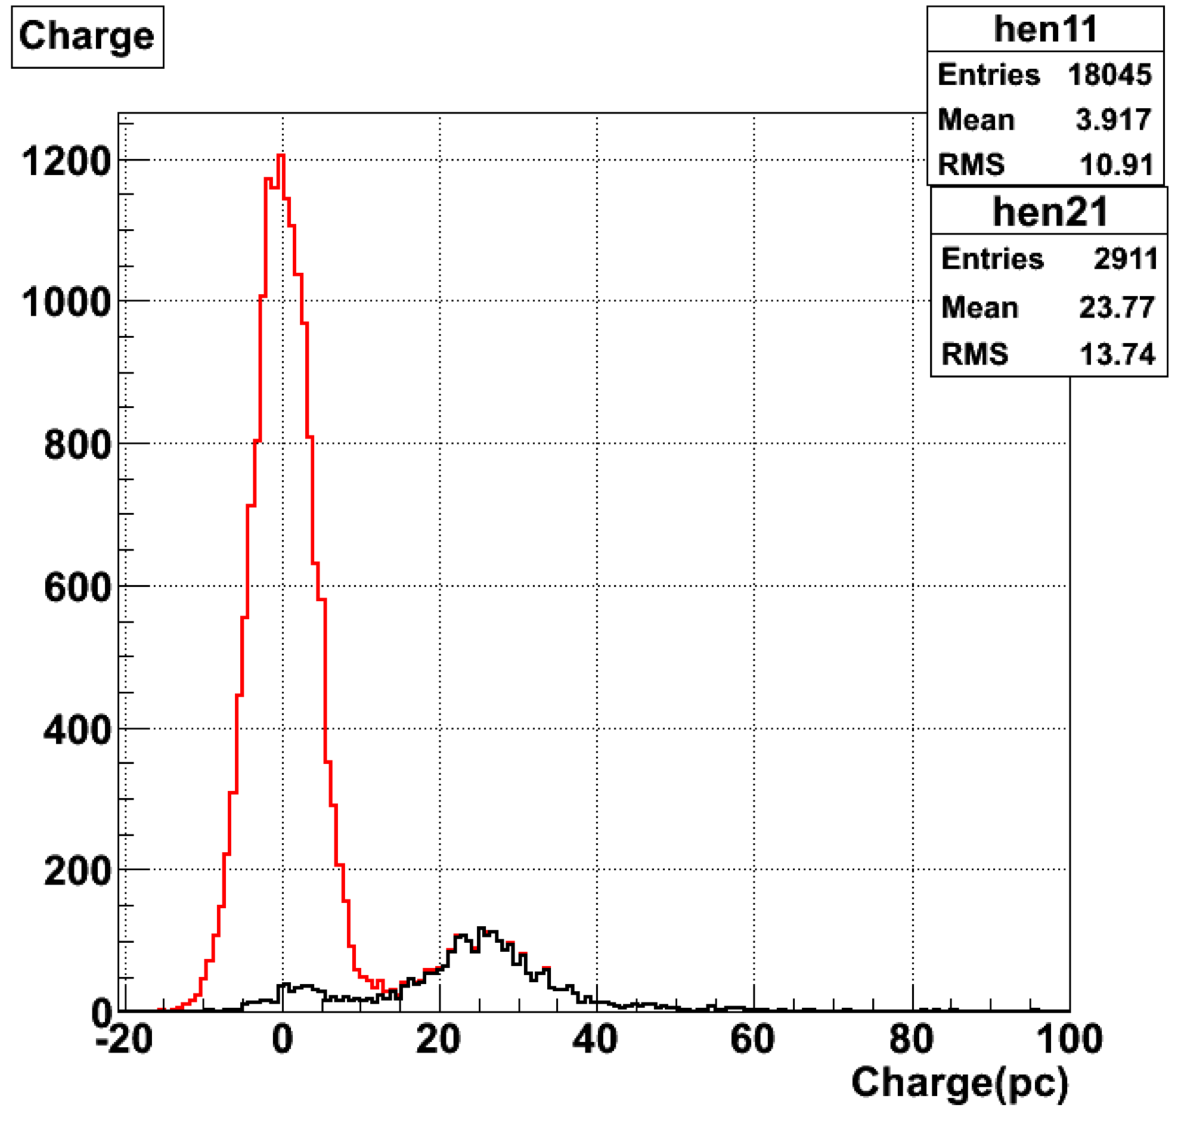
\includegraphics[scale=0.37]{ecal/MIP_10x10_APD.png}
\caption{\small{Charge distribution on QDC from readout of the HPS calorimeter crystal with Hamamatsu S8664-55 (left) and S8664-1010 (right) APDs, and the new low noise amplifier board. The red line histogram corresponds to all events, while the black line distribution is for events within $100$ ns of the trigger signal from the scintillation telescope.}}\label{fig:mip10x10}
\end{figure*}

The total cost of the replacing all ECal APDs is about $500$K\$. The HPS collaborators from IPN Orsay applied for  European Research Council (ERC) Advanced Grant 2013 to purchase APDs, for manpower costs to replace the old ones, design and build new preamplifier boards, and assemble the ECal with the new modules. This grant will include also light monitoring system. If succeeded, grant will cover most of the ECal modifications. 
